\newif\ifvimbug
\vimbugfalse

\ifvimbug
\begin{document}

\end{document}
\fi

\exercise{Optimization and Information Theory}
 

\begin{questions}

%----------------------------------------------


\begin{question}{Entropy}{5}
You work for a telecommunication company that uses a system to transmit four different symbols ${S_1, S_2, S_3, S_4}$ through time. 
In the current system, each symbol has a probability to occur according to the following table 
\begin{equation*}
\begin{array}{c|c|c|c|c}
 & S_1 & S_2 & S_3 & S_4 \\
\hline
p_i & 0.05    & 0.61    & 0.27    & 0.07
\end{array}
\end{equation*}
Compute the entropy of the system and write the minimum number of bits requires for transmission.
\begin{answer}
The minimum number of bits for transmitting the four different symbols is $N = \left\lceil\log _{2} 4\right\rceil = 2$ bits.\\
We calculate the entropy of the system to be:
\begin{equation*}
\begin{split}
H(p)=\mathbb{E}[h]=
& \quad \sum_{i} p_{i} h(p_{i})=-\sum_{i} p_{i} \log _{2} p_{i} = \\
& = - 0.05\cdot \log _{2}(0.05)  - 0.61\cdot \log _{2}(0.61)  - 0.27\cdot \log _{2}(0.27) - 0.07\cdot \log _{2}(0.07) \approx 1.43
\end{split}
\end{equation*}
\end{answer}

\end{question}

%----------------------------------------------

\begin{question}{Constrained Optimization}{25}
After an upgrade of the system, your boss asks you to change the probabilities of transmission in order to maximize the entropy. However, the new system has the following constraint
\begin{equation*}
    4 = \sum_{i=1}^4 2p_i i.
\end{equation*}
\textbf{1)} Formulate it as a constrained optimization problem. Do you need to include additional constrains beside the one above?
\\
\begin{answer}
The constrained optimization problem can be formulated as follows:
\begin{equation*}
\begin{split}
\mbox{Max }H(p_{i}) = 
&\sum_{i=1}^4 - p_{i}\log_{2}(p_i) \\
&\mbox{s.t. } \sum_{i=1}^4 2p_{i}i - 4 = 0 \\
&\qquad \sum_{i=1}^4 p_{i} - 1 = 0 \\
& \qquad p_{i} \geq 0 \qquad \forall i = 1,...,4
\end{split}
\end{equation*}
The last twi constraints are added, in order to enforce the basic rules of probability. The four probabilities have to sum to 1 and each individual probability needs to be greater or equal zero.
\end{answer}
\textbf{2)} Write down the Lagrangian of the problem. Use one Lagrangian multiplier per constraint.
\\
\begin{answer}
\begin{equation*}
\mathcal{L}(p_{i},\lambda_{1},\lambda_{2})= \sum_{i=1}^4 - p_{i}\log_{2}(p_i) + \lambda_{1}(\sum_{i=1}^4 2p_{i}i - 4)+ \lambda_{2}(\sum_{i=1}^4 p_{i} - 1)
\end{equation*}
The non-negativity constraint $ p_{i} \geq 0 \quad \forall i = 1,...,4$ is not included in the Lagrangian, because the the $\log_{2}(p_{i})$ can not take a negative argument for $p_{i}$. The non-negativity is enforced by the objective function. 
\end{answer}
\textbf{3)} Compute the partial derivatives of the Lagrangian above for each multiplier and the objective variable. Is it easy to solve it analytically? 
\\
\begin{answer}
\begin{equation*}
\begin{split}
& \frac{\partial\mathcal{L}}{\partial p_{i}}= \log_{2}(p_{i}) - \frac{1}{\log(2)}+2i\lambda_{1}+\lambda_{2} = 0 \\
& \rightarrow p_{i}^{*} = e^{-1}2^{2\lambda_{1}i+\lambda_{2}}\\ \\
& \frac{\partial\mathcal{L}}{\partial \lambda_{1}} = \sum_{i=1}^4 2p_{i}i - 4 = 0 \\
& \frac{\partial\mathcal{L}}{\partial \lambda_{2}} = \sum_{i=1}^4 p_{i} - 1 = 0
\end{split}
\end{equation*}
The problem is hard to solve analytically. We need to use the dual function to solve it.
\end{answer}
\textbf{4)} Formulate the dual function of this constrained optimization problem. Solve it analytically.
\\
\begin{answer}
The dual function is obtainned by plugging $p_{i}^{*}$ into the Lagrangian. We use the fact, that $\sum_{i=1}^4 p_{i}^{*} = 1$ for simplifying the dual function.\\
\begin{equation*}
\begin{split}
\mathcal{G}(p_{i}^{*},\lambda_{1},\lambda_{2}) &= \sum_{i=1}^4 - p_{i}^{*}\log_{2}(p_{i}^{*}) + \lambda_{1}(\sum_{i=1}^4 2p_{i}^{*}i - 4)+ \lambda_{2}(\sum_{i=1}^4 p_{i}^{*} - 1) = \\
& = \sum_{i=1}^4 - p_i^*[-1+2i\lambda_1+\lambda_2]+\lambda_1(\sum_{i=1}^4 2p_{i}i - 4) = \\
& = \sum_{i=1}^4 - p_i^*[-1+\lambda_2]-4\lambda_1 = \\
& = \sum_{i=1}^4 p_i^*-\lambda_2-4\lambda_1 = \\
& = \sum_{i=1}^4 e^{-1}2^{\lambda_2}2^{2\lambda_1i}-\lambda_2-4\lambda_1 \\
% \frac{\partial\mathcal{G}}{\partial \lambda_1} = \frac{2}{e}2^{\lambda_2}\sum_{i=1}^4i2^{\lambda_2i}-4 = 0 \\
% \frac{\partial\mathcal{G}}{\partial \lambda_1} = 
\end{split}
\end{equation*} 
We take the partial derivatives of the dual function, in order to calculate the two Langrangian multipliers and subsequently plugging them back into $p_{i}^{*}$.
\begin{equation*}
\begin{split}
& \frac{\partial\mathcal{G}}{\partial \lambda_1} = \frac{2}{e}2^{\lambda_2}\sum_{i=1}^4i2^{2\lambda_1i}-4 = 0 \qquad \rightarrow \quad  a\sum_{i=1}^4 i b^i -2 = 0 \\
& \frac{\partial\mathcal{G}}{\partial \lambda_2} = \frac{1}{e} 2^{\lambda_2}\sum_{i=1}^4 2^{2\lambda_1 i} - 1 = 0 \qquad \rightarrow \quad a\sum_{i=1}^4  b^i -1 = 0
\end{split}
\end{equation*}
We here used the substitutions $a=\frac{1}{e}2^{\lambda_2}$ and $b=2^{2\lambda_1}$.\\
by writing out the sums we obtain the following equation system for $a$ and $b$:
\begin{equation*}
\begin{split}
& a (b+2b^2+3b^3+4b^4)-2=0\\
& a (b+b^2+b^3+b^4)-1=0
\end{split}
\end{equation*} 
Solving the equation system leads to a cubic polynomial for $b$:
\begin{equation*}
-1+b^2+2b^3 = 0
\end{equation*} 
This polynomial can be solved analytically by using the following general formula for cubic equations of the form $ax^3+bx^2+c^x+d=0$. (see figure \ref{fig:cubic}) \\
By solving for the two unknowns we obtain the values of $a\approx 0.6410$ and $b\approx0.6573$.\\
 With $a$ and $b$ we can calculate the Langrangian multipliers to $\lambda_1=-0.3027$ and $\lambda_2=0.8011$.
Plugging into $p_{i}^{*}=e^{-1} 2^{2 \lambda_{1} i+\lambda_{2}}$ we can finally obtain the result to:\\ \\
$p_{1}^{*}=e^{-1} 2^{0.8011 - 2 \cdot 1 \cdot 0.3027} = 0.4213$\\
$p_{2}^{*}=e^{-1} 2^{0.8011- 2 \cdot 2 \cdot 0.3027} = 0.2770 $\\
$p_{3}^{*}=e^{-1} 2^{0.8011- 2 \cdot 3 \cdot 0.3027} = 0.1820$\\
$p_{4}^{*}=e^{-1} 2^{0.8011- 2 \cdot 4 \cdot 0.3027 }= 0.1197$
\end{answer}
\begin{figure}[h]
	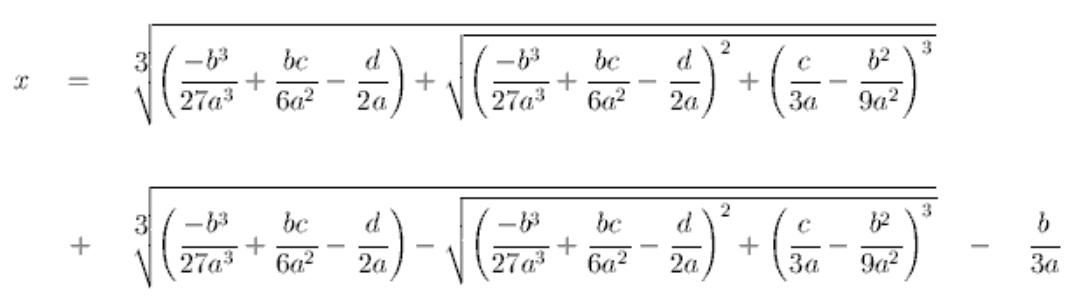
\includegraphics[width=12cm, scale=0.5]{cubics.png}
	\caption{Formula for calculating the solutions of a cubic equation. [Source: https://math.vanderbilt.edu/schectex/courses/cubic/]}
	\label{fig:cubic}
\end{figure}
\textbf{5)} Name one technique for numerically solve these problems and briefly describe it.
\begin{answer}
One method to solve constrained optimization problems numerically is the penalty method, which uses a penalty function. The goal of penalty functions is to convert constrained problems into unconstrained problems by introducing an artificial penalty for violating the constraint. This artificial penalty is added to the objective function. Now a method for unconstrained problems, like gradient descent, can be used for optimization.
\end{answer}

\end{question}
	

%----------------------------------------------

\begin{question}{Numerical Optimization}{10}
Rosenbrock's function (to be minimized) is defined as 
$$f(\boldsymbol{x}) = \sum_{i=1}^{n-1} \left[ 100 (x_{i+1} - x_{i}^{2})^{2} + (x_{i} - 1)^{2}\right].$$
Write in Python a simple gradient descent algorithm and simulate it for 10,000 steps on Rosenbrock's function with $n=20$. Attach a snippet of your algorithm, discuss the effects of the learning rate and attach a plot of your learning curve with your best learning rate.

\begin{answer}
	Choosing the right learning rate is tricky. A learning rate, which is too high, results in numerical instability and exploding gradients. A learning rate, which is too low, slows down convergence siginifigantly. From all tested cases, a learning rate of 0.0001 worked best for the given Rosenbrock function and out initialization (see figure \label{fig:LR_00001} for the learning curve). The initializations of all $x$ were drawn from a gaussian with mean $0$ and variance $0.1$. Every learning rate was tested with many initializations, in order to average out over the intializations and to find the overall best learning rate.
\end{answer}
\end{question}
\begin{figure}[h!]
	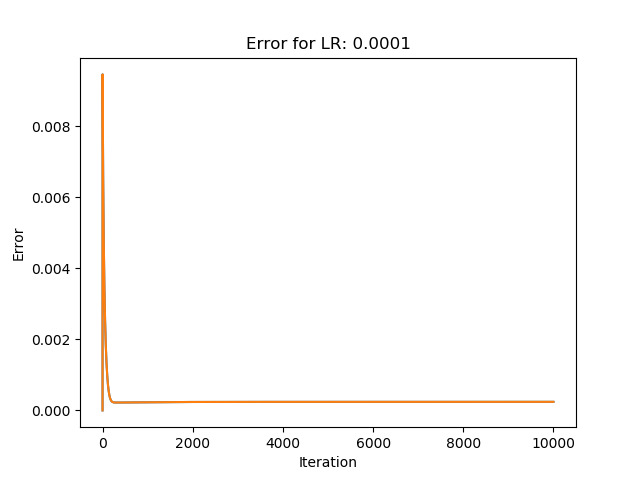
\includegraphics[width=12cm, scale=0.5]{00001.jpg}
	\caption{best learning rate was 0.0001}
	\label{fig:LR_00001}
\end{figure}
\lstinputlisting[language=Python]{gradient_descent_final.py}
%\begin{lstlisting}
%	for k in range(max_iteration):
%	    prev_x = cur_x  
%	    cur_x = prev_x - learning_rate * rosen_der(prev_x) 
%	    error = abs(cur_x - prev_x)
%	    k = k + 1 	
%	    history[k, :] = np.linalg.norm(error)
%\end{lstlisting}


%----------------------------------------------

\begin{question}{Gradient Descent Variants}{5}
Throughout this class we have seen that gradient descent is one of the most used optimization techniques in Machine Learning. This question asks you to deepen the topic by conducting some research by yourself.

\textbf{1)} There are several variants of gradient descent, namely \emph{batch, stochastic} and \emph{mini-batch}. Each variant differs in how much data we use to compute the gradient of the objective function. 
Discuss the differences among them, pointing out pros and cons of each one.

\textbf{2)} Many gradient descent optimization algorithms use the so-called \emph{momentum} to improve convergence. What is it? Is it always useful?

\begin{answer}



\textbf{Batch gradient descent} in machine learning calculates the gradient using the whole dataset. For this the computer needs to have the whole dataset in memory, which is not always doable. Because of that, its also very time consuming. It converts against the global minima of convex functions and local minima of non convex functions.

\textbf{Stochastic gradient descent} calculates the gradient for a single training example. Because of this stochastic gradient descent learns a lot faster than batch gradient descent, however its variance is very high, resulting in a highly fluctuating cost function.


\textbf{Mini-batch gradient descent} can be seen as a combination of stochastic gradient descent and batch gradient descent, using mini-batches containing $n$ training examples. This results in reduced variance and more stable conversion rate. When mini-batch gradient descent is calculated on G-PUS, it is possible to reduce the workload by using matrix operations.


\textbf{Momentum} is often used to help the gradient descent algorithm to find the global Minimum. 

Without Momentum there is a high possibility, that gradient descent starts oscillating around a local minimum. In order to reach the global minimum, this local one needs to be "jumped over". This can be interpeted as a physical impuls giving a downhill rolling sphere an impuls of energy, to help it to overcome obstacles. This "impuls" is usually calculated by looking at the last gradient and adding a part of it to the current gradient. This means, that if the last update to our parameters was big, we guess that the next one will be big, too.
\end{answer}

\begin{figure}[]
	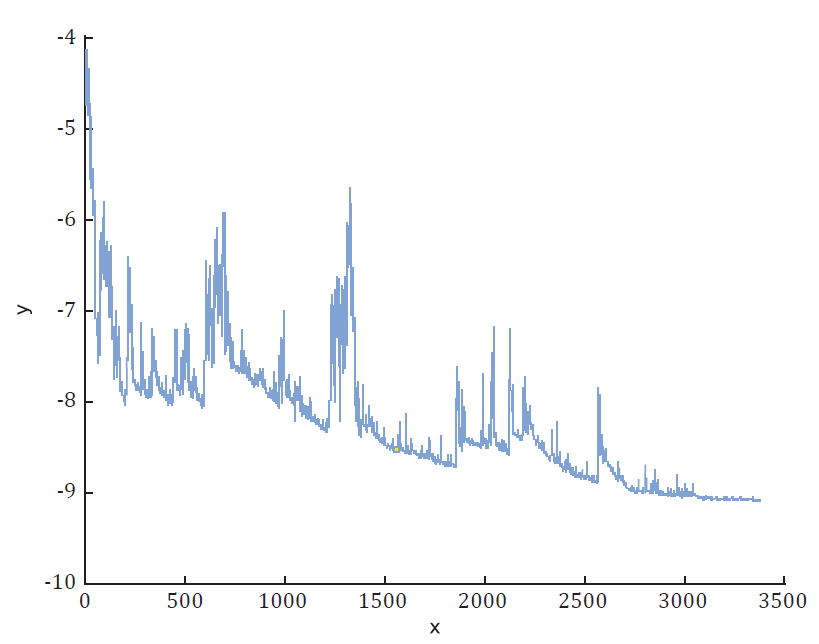
\includegraphics[width=12cm, scale=0.5]{SGD.png}
	\caption{Example for fluctuating cost function for a neural network when using SGD [Source: Me]}
	\label{fig:SGD_cost_function}
\end{figure}
\begin{figure}[]
	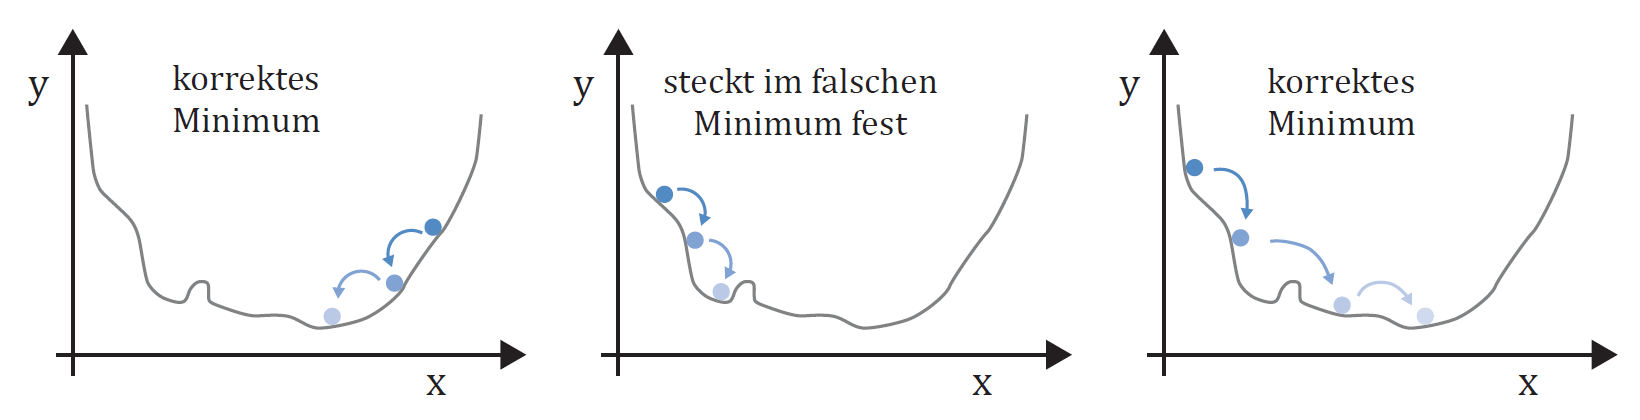
\includegraphics[width=\linewidth, scale=0.5]{momentum.png}
	\caption{Physically interpretation of Momentum [Source: Me]}
	\label{fig:Momentum}
\end{figure}


\end{question}
%----------------------------------------------

\begin{question}[bonus]{Natural Gradient}{10}
Let $\theta \in \mathbb{R}^n$ be a parameter vector
and $J \colon \mathbb{R}^n \to \mathbb{R}$ a cost function.
The negative gradient $-\nabla J(\theta)$ is sometimes called
the \emph{steepest descent direction}. But is it really?
To be able to claim that it is \emph{the} steepest descent direction,
we should compare it to other descent directions
and pinpoint what is so unique about the negative gradient direction.

\textbf{Covariant gradient.}
A fair way to compare descent directions is to make
a small step of fixed length, say $\varepsilon$,
in every direction~$\Delta \theta$ and check
which direction leads to the greatest decrease in $J(\theta)$.
Since we assume that the step size is small, we can evaluate
the decrease in $J(\theta)$ using its first-order Taylor approximation
\begin{equation*}
  J(\theta + \Delta \theta) - J(\theta) \approx
  \nabla J(\theta)^T \Delta \theta.
\end{equation*}
To make precise what we mean by \textit{small} step size,
we need to introduce a norm (or a distance)
in the space of parameters $\theta$.
A good choice, that among other advantages captures the intuition
that some parameters may influence the objective function more
than others,
is the generic quadratic norm
\begin{equation*}
  \norm{\Delta \theta}^2 =
  \frac{1}{2}\Delta \theta^T F(\theta) \Delta \theta
\end{equation*}
with a positive-definite matrix $F(\theta)$;
note that in general $F$ may depend on $\theta$.

\textbf{1)} Find the direction $\Delta \theta$ that yields
the largest decrease in the linear approximation of $J(\theta)$
for a fixed step size~$\varepsilon$.
Does this direction coincide with $-\nabla J(\theta)$?
The direction that you found is known as the
negative covariant gradient direction.
\begin{answer}
We first fomalize the optimization problem:
\begin{equation*}
\begin{aligned} \max J({\theta}+{\Delta} {\theta}) - J({\theta})& = {\nabla} J({\theta})^{T} {\Delta} {\theta} \\ \text {s.t.}&\frac{1}{2} {\Delta} {\theta}^{T} F(\theta) {\Delta} {\theta}=\varepsilon \end{aligned}
\end{equation*}
For solving this constrained optimization problem we again use the Lagrange method. We set up the Lagrangian, calculate the partial derivative of $\mathcal{L}$ for $\Delta(\theta)$ and solve for $\Delta(\theta)^*$. The last step for solving for  $\Delta(\theta)^*$ is due to the symmetry of $F(\theta)$, which follows from positive definiteness of the matrix.
\begin{align*}
\mathcal{L}(\Delta\theta,\lambda) =
&\Delta J(\theta)^T \Delta \theta + \lambda (\frac{1}{2}\Delta\theta^TF(\theta)\Delta\theta-\epsilon) \\
\frac{\partial\mathcal{L}}{\partial\Delta\theta} =& \Delta J(\theta)+ \frac{1}{2}\lambda (F(\theta)+F^T(\theta))\Delta\theta = 0 \\
\rightarrow \quad \Delta \theta^* =&- \frac{1}{\lambda}F(\theta)^{-1}\Delta J(\theta)
\end{align*}
We now can formulate the dual problem, by plugging $\Delta \theta^*$ into the Lagrangian:
\begin{align*}
\mathcal{G}(\Delta\theta^*,\lambda) &= \Delta J(\theta)^T(-\frac{1}{\lambda}F(\theta)^{-1}\Delta J)+\lambda\left[\frac{1}{2} (\frac{1}{\lambda}F(\theta)^{-1}\Delta J (\theta))^TF(\theta)(\frac{1}{\lambda}F(\theta)^{-1}\Delta J(\theta))-\epsilon\right] \\
&= -\lambda\epsilon - \frac{2}{\lambda}(\Delta J(\theta)^T F(\theta)^{-1}\Delta J(\theta))
\end{align*}
By taking the partial derivative with respect to $\lambda$ and setting the equation to zero, we can obtain $\lambda$:
\begin{align*}
\frac{\partial\mathcal{G}}{\partial\lambda}&=-\epsilon+\frac{1}{2\lambda}(\Delta J(\theta)^T F(\theta)^{-1}\Delta J(\theta))= 0  \\
&\rightarrow \lambda = \sqrt{\frac{\Delta J (\theta)^T F(\theta)^{-1} \Delta J(\theta)}{2 \epsilon}}
\end{align*}
For $\Delta \theta$ we finally obtain:
\begin{align*}
\Delta \theta = - \sqrt{\frac{\epsilon}{\Delta J(\theta)^TF(\theta)^{-1}\Delta J(\theta)}}F(\theta)^{-1}\Delta J(\theta)
\end{align*}
In this formula the term below the square root is the learning rate. The term $-F(\theta)^{-1}\Delta J(\theta)$ determines the direction of the descent. Depending on the matrix $F(\theta)^{-1}$ is not necessarily is the same direction as $-\Delta J(\theta)$, because this matrix can turn the vector to another direction.
\end{answer}
\textbf{Natural gradient.}
In statistical models, parameter vector $\theta$ often
contains parameters of a probability density function $p(x; \theta)$
(for example, mean and covariance of a Gaussian density);
thus, the cost function $J$ depends on~$\theta$ indirectly
through $p(x; \theta)$.
This two-level structure gives a strong hint to what matrix $F$
to pick for measuring the distance in the parameter space
in the most \textit{natural} way.
Namely, one can carry over the notion of `distance' between
probability distributions $p(x; \theta + \Delta \theta)$
and $p(x; \theta)$ (which is known from information theory
to be well captured by the Kullback-Leibler divergence)
to the distance between the corresponding parameter vectors
$\theta + \Delta \theta$ and $\theta$.

\textbf{2)} Obtain the quadratic Taylor approximation
of the KL divergence
from $p(x; \theta)$ to $p(x; \theta + \Delta \theta)$ in the form
\begin{equation*}
  KL(p(x; \theta + \Delta \theta) || p(x; \theta)) \approx
  \frac{1}{2}\Delta \theta^T F(\theta) \Delta \theta.
\end{equation*}
Covariant gradient with the matrix $F(\theta)$ that you found
is known as the natural gradient.

\begin{answer}\end{answer}

\end{question}



%----------------------------------------------

\end{questions}
